\documentclass[12pt,journal=tosc, notanonymous]{iacrtrans}

\usepackage[utf8]{inputenc}
\usepackage{amsmath}

\usepackage{algorithm}
\usepackage{algorithmic}
% \usepackage{amsmath} % 用于数学符号

\usepackage{amsfonts}
\usepackage{amssymb}
\usepackage{graphicx}
\usepackage{listings}
\usepackage{xcolor}
\usepackage{geometry}
\usepackage{tikz}
\usepackage{hyperref}

\definecolor{sduRed}{RGB}{163, 29, 35} 
\definecolor{sduDarkRed}{RGB}{120, 20, 25}

\usetikzlibrary{positioning, arrows.meta, shadows, calc}
\usetikzlibrary{patterns.meta}

\geometry{margin=1in}

\lstdefinestyle{cstyle}{
    language=C++,
    basicstyle=\ttfamily\small,
    keywordstyle=\color{blue}\bfseries,
    stringstyle=\color{red},
    commentstyle=\color{green},
    numbers=left,
    numberstyle=\tiny,
    stepnumber=1,
    numbersep=5pt,
    frame=single,
    breaklines=true,
    backgroundcolor=\color{gray!10}
}

\newcommand{\homework}[1]{{\color{red}{#1}}}

\hypersetup{
    colorlinks=true,
    linkcolor=blue,
    filecolor=magenta,
    urlcolor=cyan,
}

\title{Integral Attacks on Reduced Rounds of AES}
\author{Kai Hu}
\date{\today}

\begin{document}

\maketitle

% \begin{abstract}
% This report introduces the Integral Distinguisher for SmallScale AES (64-bit block cipher).
% SmallScale AES is a scaled-down version of the standard AES, using a 4x4 nibble matrix,
% GF(2$^4$) field, and a simplified round function. We provide a detailed analysis of
% the 3-round and 4-round integral distinguishers and their construction.
% \end{abstract}

\section{Introduction}

An distinguisher is used to ``distinguish'' a cipher random a random permutation (an ideal cipher). 
From an ideal cipher, you should not get any non-random information. 
That means, no matter what statistic you constructed from the input/output messages, the statistic will root from a uniform distribution.

An Integral Distinguisher is an important cryptanalysis tool, proposed by Daemen, Knudsen,
and Rijmen in 1997. Unlike differential analysis, integral analysis focuses on the
relationship of certain bits in multiple plaintexts after encryption.

In standard AES, integral distinguishers can be used to attack up to 6 rounds.
The basic integral distinguisher is a 3-round one. 



\paragraph{3-Round AES integral distinguisher.}

Encrypting a $\delta$-set of 256 messages with 3 full (with the last MC) rounds of AES, we will have a zero-sum distinguisher. 

$$
\Delta\text{-set} = \{ (x, c_1, c_2, \ldots, c_{15}): x = 0, 1, \ldots, 255 \}
$$ 

Suppose we have a set of ciphertexts, denoted by $C$. Then the zero-sum means 
$$
\bigoplus_{x \in C} x = 0
$$

The integral distinguisher of the 3-round AES can be represented as 

$$
\bigoplus_{x \in \Delta\text{-set}} F(x) = 0
$$
An illustration is shown in Figure~\ref{fig:3_round_integral_distinguisher}.


\begin{figure}[tbp!h]
\centering
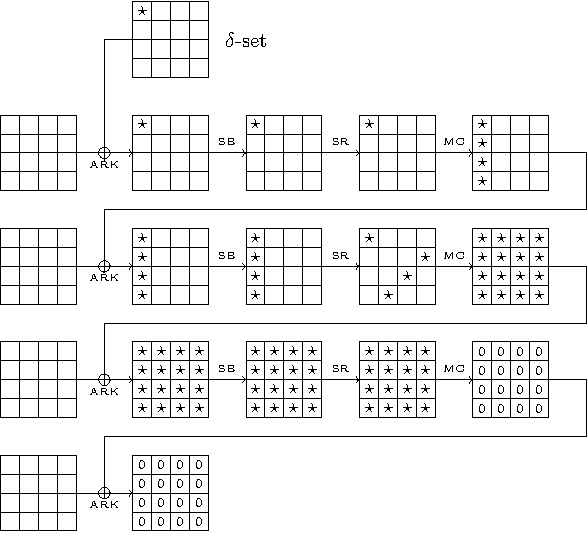
\includegraphics[width=\textwidth]{AES-3-integral.pdf}
\caption{3-Round Integral Distinguisher}
\label{fig:3_round_integral_distinguisher}
\end{figure}


\begin{proof}
The 3 rounds of AES, with the xast MC, is 
$$
F = ( AK \circ MC \circ SR \circ SB )^3 \circ AK
$$ 

A $\delta$-set is still a $\delta$-set after $SR\circ SB\circ AK$.

After the first MC and AK, the state is denoted by $w^1$, then each byte of 
$$
w^1[0], w^1[1], w^1[2], w^1[3]
$$
goes through all values, but they are related with a linear (affine) relationship. 


After the next SB and SR, they still go through all values but with a non-linear relationship.

After the next MC, AK, SB, SR, all 16 bytes go through all values, but they are non-linearly related. 

Now all 16 bytes before MC of the third round go through all values but have a non-linear relationship.

The 16 bytes can be represented by  functions of the values in the $\delta$-set.

$$
z^3[0](x), z^3[1](x), z^3[2], z^3[3](x), \ldots, z^{3}[15](x)
$$

$$
\begin{aligned}
\bigoplus_{x \in \delta\text{-set}} w^3[0] = \bigoplus_{x \in \delta\text{-set}} 2z^3[0] \oplus \bigoplus_{x \in \delta\text{-set}} 3 z^3[1] \oplus \bigoplus_{x \in \delta\text{-set}} z^3[2] \oplus \bigoplus_{x \in \delta\text{-set}} z^3[3]  
        = 0
\end{aligned}
$$
\end{proof}


\paragraph{4-Round AES integral distinguisher.}

We can construct an 4-round integral distinguisher based on the 3-round one.

\begin{figure}[H]
\centering
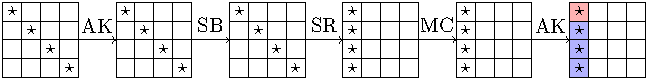
\includegraphics[width=\textwidth]{AES-4-integral.pdf}
\caption{4-Round Diagonal Integral Distinguisher}
\end{figure}


\section{Key-Recovery Attacks based on Integral Distinguishers}

Key-recovery attacks are based on the distinguishers, most usually with the ``last-round'' trick.

\begin{itemize} 
    \item If the guessed key is correct, then you have the messages to construct the distinguisher. 
    The distinguishes should hold.
    \item Otherwise, it should follow random distribution.
    \end{itemize}

See Figure~\ref{fig:key_recovery_attack_process_}.

\begin{figure}[!htbp]
\centering
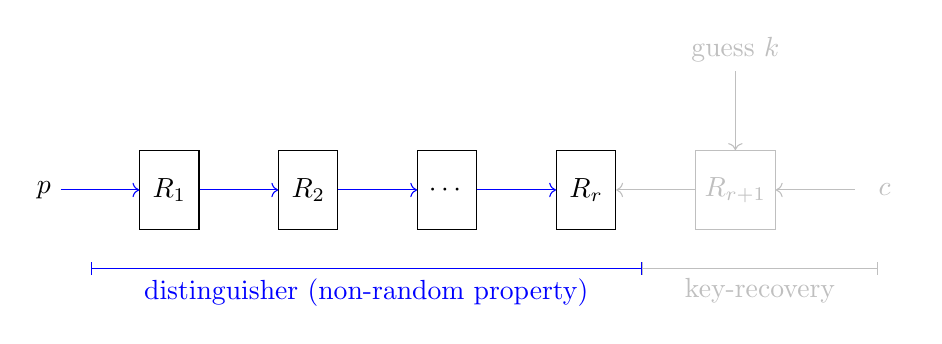
\begin{tikzpicture}
\node [rectangle, draw, minimum width=0.75cm, minimum height=1cm] (A) at (0,0) {$R_1$};
\node [rectangle, left = of A] (start) {$p$};
\node [rectangle, draw, minimum width=0.75cm, minimum height=1cm, right = of A] (B) {$R_2$};
\node [rectangle, draw, minimum width=0.75cm, minimum height=1cm, right = of B] (C) {$\cdots$};
\node [rectangle, draw, minimum width=0.75cm, minimum height=1cm, right = of C] (D) {$R_r$};
\node [rectangle, draw, minimum width=0.75cm, minimum height=1cm, right = of D, lightgray] (E) {$R_{r+1}$};
\node [rectangle, above = of E, lightgray] (k) {guess $k$};
\node [rectangle, minimum width=0.75cm, minimum height=1cm, right = of E, lightgray] (F) {$c$};

\draw [->, blue] (A) -- (B);
\draw [->, blue] (B) -- (C);
\draw [->, blue] (C) -- (D);
\draw [->, lightgray] (E) -- (D);
\draw [|-|, blue] (A)++(-1,-1) -- node[below]{distinguisher (non-random property)} ++(7,0);

\draw [->, blue] (start)-- (A);
\draw [->, lightgray] (F) -- (E);
\draw [->, lightgray] (k) -- (E);
\draw [|-|, lightgray] (A)++(-1,-1)++(7,0) -- node [below] {key-recovery} ++(3,0);


% 关键修改：终点改为 F.east，添加标注
% \draw [|-|] (start)++(0,-1) -- node[below] {distinguisher} (F.east)++(0,-1);

\end{tikzpicture}
\caption{Key-recovery attack process.}
\label{fig:key_recovery_attack_process_}
\end{figure}

\paragraph{4-round key-recovery attack.}

We collect 256 ciphertexts encrypted from a $\delta$-set after 4 rounds (without last MC).
We only need to guess the keys in the last rounds, then we can partially decrypt the 256 ciphertexts to the end of 3 full rounds. 
Since all 16 bytes of key can be split into 16 parallel functions, we can handle them one by one.
See Figure~\ref{fig:4roundkey}.

\begin{itemize}
    \item If the key byte is guessed correctly, then we reach the \underline{real} 3-round output. The distinguishers should be true.
    The correct key must pass our test.
    \item If the key is wrong, the behavior of our distinguishers should not be expected, we assume it is random. 
    That is, with $2^{-8}$ probability, a random key can pass our test. Thus, on average 1 wrong key is expected to survive.
\end{itemize} 

\begin{figure}
\centering
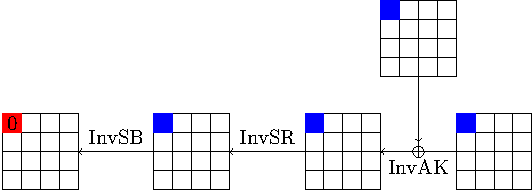
\includegraphics[width=\textwidth]{AES-3r-keyrecovery.pdf}
\caption{4-round key-recovery attack based on the 3-round distinguishers.}
\label{fig:4roundkey}
\end{figure}

\paragraph{Complexity.}
For 256 keys, we should decrypt 256 ciphertexts, the complexity is 
$
O(2^{16})
$.

\paragraph{5-round key-recovery attack based on 3-round distinguisher.}

Similar to the 4 round key recovery attacks, we can recover the last 2 round keys with the 3-round distinguisher. 
See Figure~\ref{fig:5roundkey}. The complexity is $O(2^{46})$.



\begin{figure}
\centering
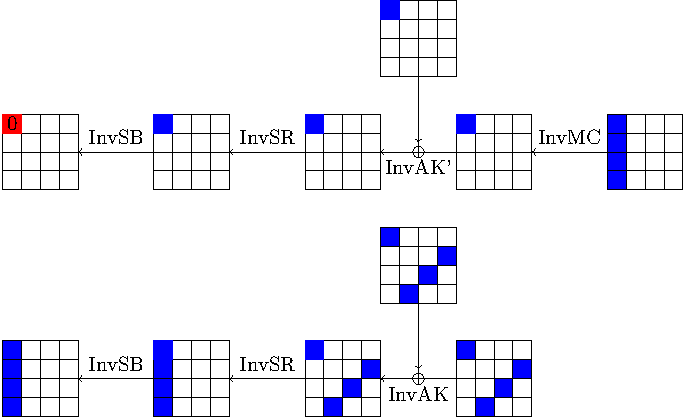
\includegraphics[width=\textwidth]{round4.pdf}
\caption{5-round key-recovery attack based on the 3-round distinguishers.}
\label{fig:5roundkey}
\end{figure}


\paragraph{5-round key-recovery attack based on 4-round distinguisher.}

Similarly, we can recover the last 1 round keys with the 4-round distinguisher. 
The complexity is $O(2^{40})$.



\paragraph{6-round key-recovery attack based on 4-round distinguisher.}

Similarly, we can recover the last 2 round keys with the 4-round distinguisher. 
The complexity is $O(2^{32+40})=O(2^{72})$.



\section{SmallScale AES Overview}

\subsection{Parameters}

SmallScale AES uses the following parameters:

\begin{itemize}
    \item Block size: 64 bits (8 bytes)
    \item State representation: 4x4 nibble matrix
    \item Key size: 64 bits (8 bytes)
    \item Irreducible polynomial: $x^4 + x + 1$ (0x13)
    \item S-box: Based on GF(2$^4$) multiplicative inverse
    % \item Number of rounds: configurable (default 5)
\end{itemize}

\subsection{Round Function Structure}

Each AES round contains four operations:

\begin{enumerate}
    \item \textbf{SubBytes (SB)}: Apply S-box to each nibble in the state
    \item \textbf{ShiftRows (SR)}: Row shifting, row $i$ shifts left by $i$ positions
    \item \textbf{MixColumns (MC)}: Column mixing using GF(2$^4$) multiplication
    \item \textbf{AddRoundKey (ARK)}: XOR with round key
\end{enumerate}

The final round does not contain MixColumns operation.

% \section{GF(2$^4$) Arithmetic}

% GF(2$^4$) multiplication is defined as follows:

% \subsection{Multiplication Operation}

% \begin{lstlisting}[style=cstyle, caption={GF(2$^4$) multiplication implementation}]
% inline uint8_t gf_mul(uint8_t a, uint8_t b) {
%     uint8_t result = 0;
%     while (b) {
%         if (b & 1) {
%             result ^= a;
%         }
%         a = a << 1;
%         if (a & 0x10) {
%             a ^= IRREDUCIBLE_POLY;  // 0x13
%         }
%         a &= 0xF;
%         b >>= 1;
%     }
%     return result;
% }
% \end{lstlisting}

Where the irreducible polynomial is $x^4 + x + 1$.

% \subsection{S-box}
The S-box is 
\begin{center}
Sbox = [6, B, 5, 4, 2, E, 7, A, 9, D, F, C, 3, 1, 0, 8]
\end{center}

There are same integral distinguishers for the SmallScaleAES.


% \homework{ Homework: Please recover the keys for the last 2 round keys, you can give some key bytes to the attacker. }

\section{Partial Sum Techniques}

Denoting the keys in the 5 round and 6 round by $K^5$ (the equivalent key after MC$^{-1}$) and $K^6$.
The ciphertext is denoted by $C$. The zero-sum byte after 4 full round is $x$. Thus,  
$$
\begin{aligned}
X = S^{-1}[ K^5[0] 
\oplus E \cdot S^{-1}[ C[0] \oplus K^6[0] ]
\oplus B \cdot S^{-1}[ C[13] \oplus K^6[13] ]\\
\oplus D \cdot S^{-1}[ C[10] \oplus K^6[10] ]
\oplus 9 \cdot S^{-1}[ C[7] \oplus K^6[7] ]
  ]
\end{aligned}
$$

Complexity: 

$$
2^{16} (2^{32} + 2^8 (2^{24} + 2^8 ( 2^{16} + 2^8 \cdot 2^8 ) ) )  \approx 2^{49} 
$$

See Algorithm~\ref{alg:key_recovery}.

\begin{algorithm}
\caption{Partial-sum algorithm for key recovery.}
\label{alg:key_recovery}
\begin{algorithmic}[1] % [1] 表示显示每一行的行号
    \REQUIRE Array $A$ of $2^{32}$ entries such that $A[j] =
    \begin{cases}
    1 & j \mbox{ appears odd times} \\
    0 & j \mbox{ appears even times}
    \end{cases}$
    \FORALL{$K^6[0], K^6[13]$} 
        \STATE Declare an empty bit-array $A_1$ of size $2^{24}$
        \FORALL{$C[0], C[13], C[10], C[7]$}
            \IF{$A[C[0], C[13], C[10], C[7]] = 1$}
                \STATE $a_1 \leftarrow E \cdot S^{-1}(C[0] \oplus K^6[0]) \oplus B \cdot S^{-1}( C[13] \oplus K^{6}[13])$
                \STATE $A_1[a_1, C[10], C[7]] \leftarrow A_1[a_1,C[10], C[7]] \oplus 1$
            \ENDIF
        \ENDFOR
        \FORALL{$K^6[10]$}
            \STATE Declare an empty bit-array $A_2$ of size $2^{16}$
            \FORALL{$a_1, C[10], C[7]$}
                \IF{$A_1[a_1, C[10], C[7]] = 1$}
                    \STATE $a_2 \leftarrow a_1 \oplus D \cdot S^{-1}(C[10] \oplus K^{6}[10])$
                    \STATE $A_2[a_2, C[7]] \leftarrow A_2[a_2,C[7]] \oplus 1$
                \ENDIF
            \ENDFOR
            \FORALL{$K^6[7]$}
                \STATE Declare an empty bit-array $A_3$ of size $2^{8}$
                \FORALL{$a_2, C[7]$}
                    \IF{$A_2[a_2, C[7]] = 1$}
                        \STATE $a_3 \leftarrow a_2 \oplus 9 \cdot S^{-1}(C[7] \oplus K^6[7])$
                        \STATE $A_3[a_3] \leftarrow A_3[a_3] \oplus 1$
                    \ENDIF
                \ENDFOR
                \FORALL{$K^5[0]$}
                    \STATE $a_4 \leftarrow 0$
                    \FORALL{$a_3$}
                        \IF{$A_3[a_3] = 1$}
                            \STATE $a_4 \leftarrow a_4 \oplus S^{-1}(K^5[0] \oplus a_3)$
                        \ENDIF
                    \ENDFOR
                    \IF{$a_4 \neq 0$}
                        \STATE $K^5[0], K^6[0], K^6[13], K^6[10], K^6[7]$ is not a valid key candidate
                    \ENDIF
                \ENDFOR
            \ENDFOR
        \ENDFOR
    \ENDFOR
\end{algorithmic}
\end{algorithm}

\section{Fast Fourier Transform}

\paragraph{Fourier transform.}

For a function $\mathbb{F}_2^n \rightarrow R$, the Fourier transform of $f$ 
is 

$$
\mathcal{F}(f)(u) = \hat{f}(u) = \sum_{x\in \mathbb{F}_2^n} (-1)^{u^\top x} f(x) 
$$  

% Example: 

We can write the function into an array 
$$
f = [f(0), f(1), \ldots, f(2^n-1)]
$$

\begin{itemize}
    \item For $u = 0$, it is equivalent to 
    $$
    \chi_0 = [(-1)^{0^\top 0}, (-1)^{0^\top 1}, \ldots, (-1)^{0^\top 2^{n}-1}] \mbox{ and } 
    \hat{f}(0) = \chi_0^\top f 
    $$
    \item For $u = 1$, it is equivalent to 
    $$
    \chi_1 = [(-1)^{1^\top 0}, (-1)^{1^\top 1}, \ldots, (-1)^{1^\top 2^{n}-1}] \mbox{ and } 
    \hat{f}(1) = \chi_1^\top f 
    $$ 
    \item .... 
    \item For $u$, it is equivalent to 
    $$
    \chi_u = [(-1)^{1^\top 0}, (-1)^{1^\top 1}, \ldots, (-1)^{1^\top 2^{n}-1}] \mbox{ and } 
    \hat{f}(1) = \chi_u^\top f 
    $$ 
    \end{itemize}

As a result, the Fourier transform is a linear transform, 
$$
\hat{f} = [\chi_u(x)]_{x, u} f 
$$

The matrix is a tensor product of a small matrix 
$$
[\chi_u(x)]_{x, u} = 
\begin{bmatrix}
1 & 1 \\
1 & -1
\end{bmatrix}^{\otimes n}
$$


\vspace{2em}
\paragraph{
The inverse of the Fourier Transform.} 

$$
\mathcal{F}^{-1}(\hat{f})(u) = f(u) = 2^{-n} \sum_{x\in \mathbb{F}_2^n} (-1)^{u^\top x} \hat{f}(x) 
$$  

The inverse of Fourier transform is also a matrix multiplication, which is also a tensor of a small matrix.

$$
[\chi_u(x)]_{x, u}^{-1} = 
\Big(
\frac{1}{2}\begin{bmatrix}
1 & 1 \\
1 & -1
\end{bmatrix}
\Big)
^{\otimes n}
$$

\paragraph{Fast Algorithm.}

A matrix multiplication with a vector requires $2^{2n}$ complexity. We can reduce it to $O(n2^n)$
if the matrix is a tensor of a small matrix.

Let $M = H^{\otimes n} = \begin{bmatrix} a_0 & a_1 \\ a_2 & a_3 \end{bmatrix}^{\otimes n}$.
For $x: \mathbb{F}_2^n \rightarrow \mathbb{R}$,

$$
\begin{aligned}
M x = 
\begin{bmatrix}
a_0 H^{\otimes n-1} & a_1 H^{\otimes n-1} \\ 
a_2 H^{\otimes n-1} & a_3 H^{\otimes n-1} \\ 
\end{bmatrix}
\cdot 
\begin{bmatrix}
x_H\\
x_L
\end{bmatrix} 
= 
\begin{bmatrix}
a_0 H^{\otimes n-1}  x_H \oplus a_1 H^{\otimes n-1} x_L \\ 
a_2 H^{\otimes n-1}  x_H \oplus a_3 H^{\otimes n-1} x_L 
\end{bmatrix}
% = 
% \begin{bmatrix}
% H^{\otimes n-1} (a_0 x_H \oplus a_1 x_L) \\ 
% H^{\otimes n-1} (a_2 x_H \oplus a_3 x_L) 
% \end{bmatrix}
\end{aligned}
$$
See Figure~\ref{fig:tensor}.

The algorithm is 

% \documentclass{article}

% % 导入必要的宏包
% \usepackage{algorithm}
% \usepackage{algorithmic}
% \usepackage{amsmath} % 用于数学符号
% \usepackage{geometry} % 用于调整页边距，防止代码过宽

% \geometry{a4paper, margin=1in}

% \begin{document}

\begin{algorithm}[H]
\caption{Walsh transform algorithm}
\label{alg:walsh_transform}
\begin{algorithmic}[1] % [1] 表示显示行号
    \REQUIRE Input Table $T$ containing $2^n$ elements $-1, 1$
    % \COMMENT{Variable Sz is the small table size}
    % \COMMENT{Variable Pos is the small table position}

    \FOR{$i$ from $0$ to $n-1$}
        \STATE Let $\text{Sz} \leftarrow 2^i$, $\text{Pos} \leftarrow 0$
        \WHILE{$(\text{Pos} < 2^n)$}
            \FOR{$j$ from $0$ to $\text{Sz} - 1$}
                \STATE Let $\text{Sum} \leftarrow T[\text{Pos} + j] + T[\text{Pos} + \text{Sz} + j]$
                \STATE Let $\text{Diff} \leftarrow T[\text{Pos} + j] - T[\text{Pos} + \text{Sz} + j]$
                \STATE $T[\text{Pos} + j] \leftarrow \text{Sum}$
                \STATE $T[\text{Pos} + \text{Sz} + j] \leftarrow \text{Diff}$
            \ENDFOR
            \STATE Let $\text{Pos} \leftarrow \text{Pos} + 2 \cdot \text{Sz}$
        \ENDWHILE
    \ENDFOR

    \STATE Output overwritten content of $T$ containing $W(T)$
\end{algorithmic}
\end{algorithm}


% \paragraph{Homework}

\homework{Homework: Implement this algorithm.}



\begin{figure}
\centering
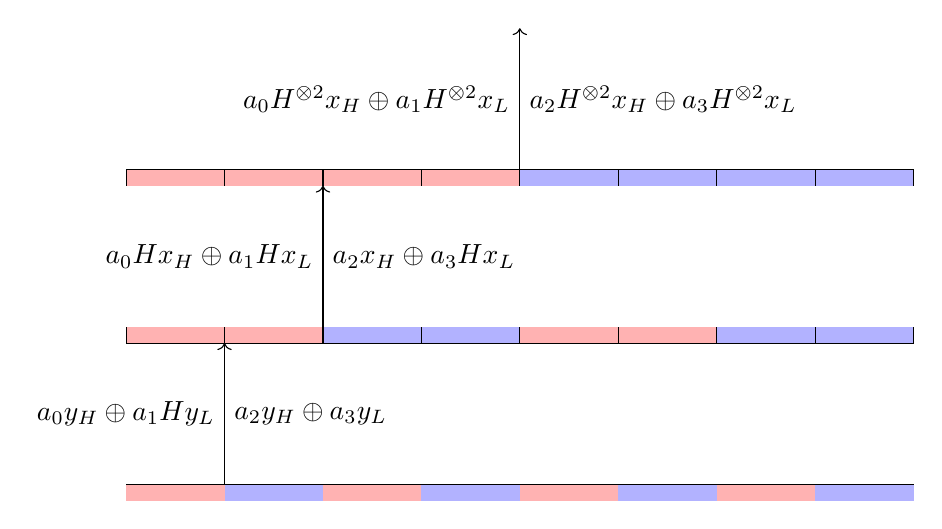
\begin{tikzpicture}

\draw (0,0) rectangle ++(10, 0.2);
\fill [red!30] (0,0) rectangle ++(5, 0.2);
\fill [blue!30](5,0) rectangle ++(5, 0.2);
\draw [->] (5, 0.2) -- node[left]{$a_0 H^{\otimes 2} x_H \oplus a_1 H^{\otimes 2} x_L$} node [right] {$a_2 H^{\otimes 2} x_H \oplus a_3 H^{\otimes 2} x_L$} ++(0, 1.8);

\draw (0, 0)  -- ++(0, 0.2);
\draw (1.25, 0)  -- ++(0, 0.2);
\draw (2.50, 0)  -- ++(0, 0.2);
\draw (3.75, 0)  -- ++(0, 0.2);
\draw (5.00, 0)  -- ++(0, 0.2);
\draw (6.25, 0)  -- ++(0, 0.2);
\draw (7.50, 0)  -- ++(0, 0.2);
\draw (8.75, 0)  -- ++(0, 0.2);
\draw (10.00, 0)  -- ++(0, 0.2);

\begin{scope}[yshift=-2cm]
\draw (0,0) rectangle ++(10, 0.2);
\fill [red!30] (0,0) rectangle ++(2.5, 0.2);
\fill [blue!30] (2.5,0) rectangle ++(2.5, 0.2);
\fill [red!30](5,0) rectangle ++(2.5, 0.2);
\fill [blue!30](7.5,0) rectangle ++(2.5, 0.2);

\draw (0, 0)  -- ++(0, 0.2);
\draw (1.25, 0)  -- ++(0, 0.2);
\draw (2.50, 0)  -- ++(0, 0.2);
\draw (3.75, 0)  -- ++(0, 0.2);
\draw (5.00, 0)  -- ++(0, 0.2);
\draw (6.25, 0)  -- ++(0, 0.2);
\draw (7.50, 0)  -- ++(0, 0.2);
\draw (8.75, 0)  -- ++(0, 0.2);
\draw (10.00, 0)  -- ++(0, 0.2);

\draw [->] (2.5, 0.2) -- node[left]{$a_0 H x_H \oplus a_1 H x_L$} node [right] {$a_2 x_H \oplus a_3 H x_L$} ++(0, 1.8);

\end{scope}




\begin{scope}[yshift=-4cm]
\draw (0,0) rectangle ++(10, 0.2);
\fill [red!30] (0,0) rectangle ++(1.25, 0.2);
\fill [blue!30] (1.25,0) rectangle ++(1.25, 0.2);
\fill [red!30] (2.5,0) rectangle ++(1.25, 0.2);
\fill [blue!30] (3.75,0) rectangle ++(1.25, 0.2);

\fill [red!30](5,0) rectangle ++(1.25, 0.2);
\fill [blue!30](6.25,0) rectangle ++(1.25, 0.2);
\fill [red!30](7.5,0) rectangle ++(1.25, 0.2);
\fill [blue!30](8.75,0) rectangle ++(1.25, 0.2);

\draw [->] (1.25, 0.2) -- node[left]{$a_0 y_H \oplus a_1 H y_L$} node [right] {$a_2 y_H \oplus a_3 y_L$} ++(0, 1.8);


\end{scope}


% \begin{scope}[yshift=-6cm]
% \draw (0,0) rectangle ++(10, 0.2);
% \fill (0,0) rectangle ++(1.25, 0.2);
% \fill [blue!30] (1.25,0) rectangle ++(1.25, 0.2);
% \fill [red!30] (2.5,0) rectangle ++(1.25, 0.2);
% \fill [blue!30] (3.75,0) rectangle ++(1.25, 0.2);

% \fill [red!30](5,0) rectangle ++(1.25, 0.2);
% \fill [blue!30](6.25,0) rectangle ++(1.25, 0.2);
% \fill [red!30](7.5,0) rectangle ++(1.25, 0.2);
% \fill [blue!30](8.75,0) rectangle ++(1.25, 0.2);

% \draw [->] (1.25, 0.2) -- node[left]{$a_0 z_H \oplus a_1 z_L$} node [right] {$a_2 z_H \oplus a_3 z_L$} ++(0, 1.8);
% \end{scope}

\end{tikzpicture}
\caption{Illustration of the 3-bit tensor matrix multiplication.}
\label{fig:tensor}
\end{figure}





\paragraph{Convolution.}
For two functions $f, g: \mathbb{F}_2^n \rightarrow R$, the convolution is defined as 
$$
(f \star g) (u) = \sum_{x \in \mathbb{F}_2^n} f(x) g(x \oplus u) 
$$
The normal way to compute $(f \star g)[u]$ for all $u \in \mathbb{F}_2^n$ requires $O(2^{2n})$ complexity.
But we have a quicker way that needs only $O(n2^{n})$.

\begin{enumerate}
    \item Apply Fourier transform to $f$ and $g$ to get $\hat{f}$ and $\hat{g}$
    \item Compute $f \odot g$ (element-wise product)
    \item Apply the inverse Fourier transform to $\mathcal{F}^{-1}(f \odot g)$.
    \end{enumerate}

\begin{proof}
Denoting $z: \mathbb{F}_2^n \rightarrow \mathbb{R}$ as the convolution of $f$ and $g$, i.e., 
$$
z(u) = (f \star g) (u) = \bigoplus_{x \in \mathbb{F}_2^n} f(x) g(x \oplus u).
$$
Applying the Fourier transform to $z$, we get 
$$
\begin{aligned}
( \mathcal{F}^{-1} z )[v] &= \sum_{t \in \mathbb{F}_2^n} (-1)^{v^\top t} \sum_{x \in \mathbb{F}_2^n} f(x) g(x \oplus v) \\
 &= \sum_{x \in \mathbb{F}_2^n} f(x) \sum_{y \in \mathbb{F}_2^n} (-1)^{v^\top (y\oplus x)}  g(y)\\
 &= \sum_{x \in \mathbb{F}_2^n} (-1)^{v^\top x} f(x) \sum_{y \in \mathbb{F}_2^n} (-1)^{v^\top y} g(y) \\
 & = ( \mathcal{F} f )[v] \cdot  ( \mathcal{F} g )[v]
\end{aligned}
$$
Thus, 
$$
z = \mathcal{F}^{-1} ( ( \mathcal{F} f ) \odot  ( \mathcal{F} g ) )
$$
\end{proof}

\homework
{
Homework: 
Generate a random function $f: \mathbb{F}_2^{16} \rightarrow \mathbb{R}$ and $g: \mathbb{F}_2^{16} \rightarrow \mathbb{R}$.
Compute 
$$
z = f \star g 
$$
using the convolution method.
}

\section{FFT in Integral Attacks}
Suppose we have guess $K^5[0]$. For each the guess, consider one bit of $X$, e.g., $h$, 

Generating a vector $f \in \mathbb{F}_2^{32}$ with $x = (C[0], C[13], C[10], C[7])$ as the index, and 
$$
f(x) = 
\begin{cases}
1 & C[0], C[13], C[10], C[7] \mbox{ appears odd times } \\
0 & C[0], C[13], C[10], C[7] \mbox{ appears even times } \\
\end{cases}
$$ 

Let $g: \mathbb{F}_2^{32} \rightarrow \mathbb{R}$, and denote $k = (K^6[0], K^6[13], K^6[10], K^6[7])$.
$$
g(x \oplus k) 
= 
\begin{cases}
1 & \mbox{ if $x$ and $k$, and $K^5[0]$ can lead to $h = 1$ }\\
0 & \mbox{ if $x$ and $k$, and $K^5[0]$ can lead to $h = 0$ }\\
\end{cases}
$$
Thus, the value of $X[0]$ can be compute 
$$
h = \sum_{x \in \mathbb{F}_2^{32}} f(x) g(x \oplus k) = \mathcal{F}^{-1} ( \mathcal{F}(f) \odot \mathcal{F}(g) ) 
$$

Time complexity: 
$$
O( 8 \cdot 2^{8} \cdot 4 \cdot 2^{32} \times 32 ) \approx 2^{50}
$$

\homework{Homework} Using partial-sum or FFT, please recover the last 2 rounds of keys for SmallScaleAES based on the 4-round integral distinguisher. 


\end{document}
